\subsection{Lecture 6: Definiteness, Isometries and Adjoints}
\subsubsection{Classification of Bilinear Forms: Symmetric Bilinear Forms Part 2}
\begin{defn}
\index{Symmetric!Bilinear Form!Positive (Semi)Definite}
\index{Symmetric!Bilinear Form!Negative (Semi)Definite}
Let $V$ be a finite dimensional vector space over $\RR$. Let $G$ be a symmetric bilinear form and let $Q(v)=G(v,v)$. 
    \begin{itemize}
    \item {
    $G$ is positive definite if $Q(v)>0$ for all $v\in V$.
    }
    \item {
    $G$ is negative definite if $Q(v)<0$ for all $v\in V$.
    }
    \item {
    $G$ is non-negative (positive semidefinite) if $Q(v)\geq 0$ for all $v\in V$.
    }
    \item {
    $G$ is non-positive (negative semidefinite) if $Q(v)\leq 0$ for all $v\in V$
    }
    \item {
    $G$ is indefinite if there exists some $v,w\in V$ so that $Q(v)>0, Q(w)<0$. 
    }
    \end{itemize}
\end{defn}

By Sylvester's theorem, there is a basis $B = \{e_1,...,e_p,f_1,...,f_q,g_1,...,g_{n-p-q}\}$ where $[G]_B = \diag(1,...,1,-1,...-1,0,...,0)$, with $p$ ones, $q$ minus ones, and $n-p-q$ zeros. 
\begin{remark*}
    $G|_{\Span\{e_1,...,e_p\}}$ is positive definite and
    $G|_{\Span\{f_1,...,f_q\}}$ is negative definite.
\end{remark*}
\begin{remark*}
    $G$ is positive definite if and only if $p=n$, negative definite if and only if $q=n$, and indefinite if and only if $q>0$ and $p>0$. If $n-p-q>0$ then $G$ is degenerate. $G$ is nonpositive iff $p=0$, and $G$ is nonnegative iff $q=0$. If $G$ is nondegenerate then the signature $(p,q)$ is well defined.
\end{remark*}
\begin{remark*}
    The space $\Span\{e_1,...,e_p\}$ might depend on the choice of basis (ie. different bases can give different hyperplanes, but $G$ is still positive definite on these hyperplanes). Only the dimension is invariant of the basis.
\end{remark*}

\begin{example}
    Consider $V = \RR^2$ and let $S=\{e_1,e_2\}$ be the standard basis. Let $v = ae_1 + be_2$. That is, $[v]_S = (a,b)$. But in the standard basis we usually just write $v=(a,b)$ since it is understood what basis we mean. 
    
    Set,
    \[[G]_S= \m{1&0\\0&-1}\]
    Then, 
    \[Q(v) = [v]_S^T [G]_S [v]_S = \m{a\\b}^T\m{1&0\\0&-1}\m{a\\b} = a^2-b^2\]
    That is, $Q(ae_1+be_2) = a^2-b^2$. 

    Now consider the vectors $u_1 = (1,1)$ and $u_2 = (1,-1)$. Let $U_1 = \Span\{u_1\}$ and $U_2 = \Span\{u_2\}$. Let $\lambda \in \RR$ be any real number. We can see that $Q(\lambda u_1) = \lambda^2(1-1) = 0$, and $Q(\lambda u_2) = \lambda^2(1-1)=0$. Therefore $G|_{U_1}=0$ and $G|_{U_2}=0$. 

    Similarly, for any $v_1 = (1,\epsilon)$ with $-1<\epsilon < 1$, we have $Q(\lambda v_1) > 0$. For $v_2 = (\epsilon,1)$ with $-1<\epsilon<1$ we have $Q(\lambda v_2)<0$. This allows us to draw a diagram of the regions where $G$ is positive and negative definite.
    \label{example:quadraticform}
\end{example}
\begin{figure}[h]
        \centering
        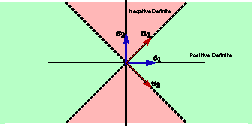
\includegraphics[width=0.95\linewidth]{quadraticformr2.pdf}
        \caption{Diagram showing the regions where $Q$ from example \ref{example:quadraticform} is positive and negative definite, as well as the two lines where it is zero.}
        \label{fig:quadform}
\end{figure}
\begin{remark*}
    In example \ref{example:quadraticform}, we saw that the region where $G$ is positive or negative definite, are not lines through $\RR^2$, and instead they form a kind of flat cone shaped region. Each region consists of infinitely many lines, on which $G$ can be restricted in order to get a positive or negative definite form. In summary, there is no unique subspace $V_0$ of $\RR^2$ where $G|_{V_0}$ is positive definite, and the same can be said for negative definite.
\end{remark*}

\subsubsection{Isometries} 
A nice way to classify bilinear forms is through their set of isometries. Isometries are transformations on $V$ which preserve the bilinear form, and isometry of vector spaces forms an equivalence relation.
\begin{defn}[Pullback of Bilinear Form] \index{Bilinear Form!Pullback}Let $V$ be an $n$ dimensional vector space over a field $\FF$ of characteristic zero. Let $G$ be a nondegenerate symmetric bilinear form on $V$. Let $W$ be some other vector space over $\FF$ and consider a linear map $P : W\to V$. Then we define the \textbf{pullback of $G$ with respect to $P$} to be a bilinear form $P^* G$ on $W$ defined by 
\begin{equation}P^* G(w_1,w_2) = G(P(w_1),P(w_2))\end{equation}
\end{defn}
\begin{defn}[Isometry]\index{Isometry} Let $V_1,V_2$ be two vector spaces, and let $G_1,G_2$ be nondegenerate symmetric bilinear forms on $V_1$ and $V_2$ respectively. Then a map $P : V_1 \to V_2$ is called an \textbf{isometry} if $P^* G_2 = G_1$. 
\end{defn}
\begin{lemma}
    Let $\dim V_1 = \dim V_2$. Then any isometry between $V_1$ and $V_2$ is an isomorphism.
\end{lemma}
\begin{proof}
     Let $v_1\in \ker P$. Then $G_1(v_1,v_2) = G_2(P(v_1),P(v_2))=0$ forall $v_2$. But since $G_1$ is nondegenerate, this is true forall $v_2$ iff $v_1 = 0$. So $v_1=0$ for all $v_1 \in \ker P$. Thus $\ker P = \{0\}$ and so we are done.
\end{proof}
\begin{defn}\index{Isometric}
    Let $V_1,G_1$ and $V_2,G_2$ be vector spaces with nondegenerate symmetric bilinear forms. We say $V_1$ is \textbf{isometric} to $V_2$ if there exists an isometry between them.
\end{defn}
\begin{remark*}
    Isometry is an equivalence relation.
\end{remark*}

\begin{defn}[Orthogonal Group]\index{Group!Orthogonal}\index{Orthogonal!Group} Let $V$ be a vector space and let $G$ be a metric on $V$. The set of all isometries $P : V\to V$ with $P^* G = G$ is a subgroup of $L(V)$ called the \textbf{orthogonal group} and we denote it $\Orth(V,G)$. 
\begin{equation}
    \Orth(V,G) = \{P \in L(V): P^* G= G\}
\end{equation}
\end{defn}
\begin{remark*}
    If $G$ is of signature $(p,q)$ we often write this as $\Orth(p,q,V)$.

    If the vector space is $V=\RR^n$, and $G$ is of signature $(n,0)$ we just write $\Orth(n,\RR)$.
\end{remark*}
\begin{defn}
    \index{Group!Special Orthogonal}
The \textbf{special orthogonal group} $\SO(V,G)$ is the set of all orthogonal transformations $T\in \Orth(V,G)$ with $\det T = 1$.
\end{defn}
\begin{remark*}
An isometry of $V,G$ is sometimes called an orthogonal transformation.
\end{remark*}
\begin{lemma}
    Let $B$ be a basis of $V$. Then $P$ is an isometry of $G$ iff $[P]_B^T[G]_B[P]_B = [G]_B$.
\end{lemma}
\begin{proof}
    Recall that $G(v,w) = [v]_B^T [G]_B[w]_B$. Then \begin{align*}G(P(v),P(w)) &= ([P]_B[v]_B)^T[G]_B[P]_B[w]_B \\&= [v]_B[P]_B^T[G]_B[P]_B[w]_B\end{align*}
    So we need $[P]_B^T[G]_B[P]_B = [G]_B$.
\end{proof}
\subsubsection{Adjoints}
\begin{lemma}
Let $V$ be a finite dimensional vector space over a field $\FF$ of characteristic $0$. Let $G$ be a symmetric or skew nondegenerate bilinear form on $V$. Let $B$ be any other bilinear form on $V$. Then there exists a unique linear map $T_B : V\to V$ so that $B(v,w) = G(T_B(v),w)$ for all $v,w$.
\end{lemma}
\begin{proof}
    Recall the flat map, $\flat_G : V \to V^*$ defined by $\flat_G(v)(w) = G(v,w)$. We know $\flat_G$ is an isomorphism since $G$ is nondegenerate. Let $\flat_B(v)(w) = B(v,w)$ as well. So $B(v,w)=G(T_B(v),w)$ iff $\flat_B(v)(w)=\flat_G(T_B(v))(w)$ for all $w$, if and only if $\flat_B = \flat_G\circ T_B$. So we just have to set $T_B = \flat_G^{-1}\circ \flat_B$. Since $\flat_G$ is an isomorphism and hence invertible, this definition is perfectly good. 
\end{proof}
\begin{remark*}
    So given a fixed nondegnerate bilinear form $G$ on $V$ we have an isomorphism $\iota$ between $V^* \otimes V^*$ and $V\otimes V^*$, given by $\iota(B) = T_B$ as above. 
\end{remark*}
\begin{defn}[Adjoint] Let $G$ be a nondegenerate bilinear form on $V$ (symmetric or skew). For any map $T : V \to V$ we define a linear map $T^\dagger : V \to V$ by the formula $G(v,T(w)) = G(T^\dagger(v),w)$ for all $v,w\in V$. $T^\dagger$ is called the \textbf{adjoint} of $T$.
\end{defn}
\begin{remark*}
    $T^\dagger$ is not the same as the dual map $T^*$. But they are related by a formula.
\end{remark*}
\begin{lemma}
    The map $T^\dagger$ is the only map satisfying $G(v,T(w))=G(T^\dagger(v),w)$ for all $v,w$.
\end{lemma}
\begin{proof}
    Let $B \in V^*\otimes V^*$ where $B(v,w)=G(v,Tw)$. Then there is a unique map $T_B : V\to V$ given by $B(v,w) = G(T_B(v),w)$. Therefore we have $G(T_B(v),w)=G(v,T(W))$ so $T_B = T^\dagger$ as required.
\end{proof}
\begin{remark*}
    Since $G$ is either skew or symmetric, $
G(v,Tw) = G(T^\dagger v,w)$ implies that $\pm G(T(w),v) = \pm G(w,T^\dagger V)$. So $G(T(v),w) = G(v,T^\dagger(w))$. Therefore $T$ satisfies the same definition as $(T^\dagger)^\dagger$. Since adjoints are unique, $T = (T^\dagger)^\dagger$.

It also follows that $(T\circ S)^\dagger = S^\dagger\circ T^\dagger$.
\end{remark*}
\begin{remark*}
    The dual map and the adjoint are related. Observe, $G(v,T(w)) = G(T^\dagger (v),w)$, so $\flat_G(v)(T(w)) = \flat_G(T^\dagger(v))(w)$. But $\flat_G(v)(T(w)) = T^*\flat_G(v)(w)$, so $T^*(\flat_G) = \flat_G \circ T^\dagger$. Hence,
    \begin{equation}
        T^\dagger = \flat_G^{-1} \circ T^*(\flat_G) = \sharp_G\circ T^*\circ \flat_G
    \end{equation}
\end{remark*}

\begin{defn}[Self/Skew-Adjoint]\index{Operator!Self-Adjoint}\index{Operator!Skew-Adjoint} A map $T : V \to V$ is called self-adjoint if $T^\dagger = T$. It is called skew-adjoint if $T=-T^\dagger$.
\end{defn}
\begin{remark*}
    Let $T \in L(V)$. Then we can write $T = \frac{1}{2}(T+T^\dagger)+\frac{1}{2}(T-T^\dagger)$. Observe that $\frac{1}{2}(T+T^\dagger)$ is self adjoint and $\frac{1}{2}(T-T^\dagger)$ is skew-adjoint!
\end{remark*}
\begin{lemma}
    $B$ is symmetric iff $T_B$ is self-adjoint, and $B$ is skew iff $T_B$is skew-adjoint.
\end{lemma}
\begin{proof}
    Let $B \in V^*\otimes V^*$ and let $T_B \in \End(V)$. We have $B(v,w) = G(T_B(v),w) = G(v,T_B^\dagger(w)) = \pm G(T^\dagger(w),v)$. Suppose $G$ is symmetric. Then $B(v,w) = G(T^\dagger_B(w),v) = G(T_B(w),v)$ for all $v,w$. Since $G$ is nondegenerate, we have $T^\dagger_B(w)=T_B(w)$ for all $w$. This means $T_B$ is self adjoint. 

    For the other direction, we see that if $T_B$ is self adjoint then $B(v,w) = G(T_B(v),w) = G(w,T_B(v)) = B(w,v)$. 

    If we did this proof again for skew $G$, then we would have a minus sign everywhere. Therefore the proof for skew-adjoint $T_B$ is identical.
\end{proof}

\subsection{Lecture 7: Reflections, Hyperbolic Planes, and Cancellation}

\subsubsection{Adjoint Basis}
For all of this lecture, $V$ is a finite dimensional vector space over a field $\FF$ of characteristic zero, and $G$ is a symmetric bilinear form.

Recall that $\flat : V \to V^*$ and $\flat(v)(w) = G(v,w)$. Let $B = \{e_1,...,e_n\}$ and $B^* = \{e^1,...,e^n\}$.
Let $\flat(e_i) = A_{ij} e^j$. Observe that $\flat(e_i)(e_j) = G_{ij} = A_{ij}$. So $[\flat]_{B^* B} = [G]_B$.
\begin{defn}[$G$-adjoint Basis]\index{Basis!G-adjoint}The set $\{\flat(e_i) : i =1,...,n\}$ is a basis for $V^*$ called the $G$-adjoint basis. We denote it by $B^\dagger$.\end{defn}
\begin{remark*}
    If $B$ is an orthonormal basis then $B^* = B^\dagger$. In this basis $[T]^\dagger_B = [T]^T_B$.
\end{remark*}

\subsubsection{Classification of Bilinear Forms: Symmetric Bilinear Forms Part 3}
The problem is to classify all symmetric nondegenerate bilinear forms (metrics) on $V$. Given a vector space $V$, can we classify all possible metrics up to isometry (that is, we only say two metrics are different if we can not transform one into another via an isometry). This classification will be based off the proof in the book Basic Algebra I by Jacobson \cite{Jacobson2009-pp}.

\begin{defn}[Reflection]\index{Reflection} Let $v$ be a vector which is not isotropic, so $Q(v)\neq 0$. Then we define a linear map $R_v : V \to V$ by $R_v(u) = u-2\frac{G(u,v)}{Q(v)}v$. This map is called a \textbf{reflection generated by $v$}
\end{defn}
\begin{remark*}
    $R_{tv} = R_v$ for all $t\in\RR$
\end{remark*}
\begin{lemma}
 The map $R_v$ is an isometry.   
\end{lemma}
\begin{proof}
    By the polarization identity, the map $R_v$ is an isometry iff $Q(R_v(u))=Q(u)$ for all $u\in V$. We have
    \begin{align*}
        Q(R_v(u))&=Q\left(u-2\frac{G(u,v)}{Q(v)}v\right)\\
        &= G\left(u-2\frac{G(u,v)}{Q(v)}v,u-2\frac{G(u,v)}{Q(v)}v\right)\\
        &= Q(u) - 4\frac{G(u,v)G(v,u)}{Q(v)}+4\frac{G(u,v)^2G(v,v)}{Q(v)}\\
        &= Q(u)
    \end{align*}
    Where we have used the fact that $G$ is symmetric to cancel out the last two terms. 
\end{proof}

\begin{remark*}
    Let $u \in \Span\{v\}^\perp$. Then $G(u,v)=0$, so $R_v(u)=u$.
\end{remark*}
\begin{remark*}
    Suppose $u=v$. Then $R_v(u) = v-2v = -v$.
\end{remark*}
\begin{remark*}
    Based on the above two facts, we observe that $R_v$ is a reflection over the hyperplane $\Span\{v\}^\perp$.
\end{remark*}
\begin{example}
    Let $V = \RR^3$ and let $G$ be the standard inner product, $G(v,w) = v^1 w^1 + v^2 w^2 + v^3 w^3$. We have the following picture. 
\end{example}
\begin{figure}[h!]
    \centering
    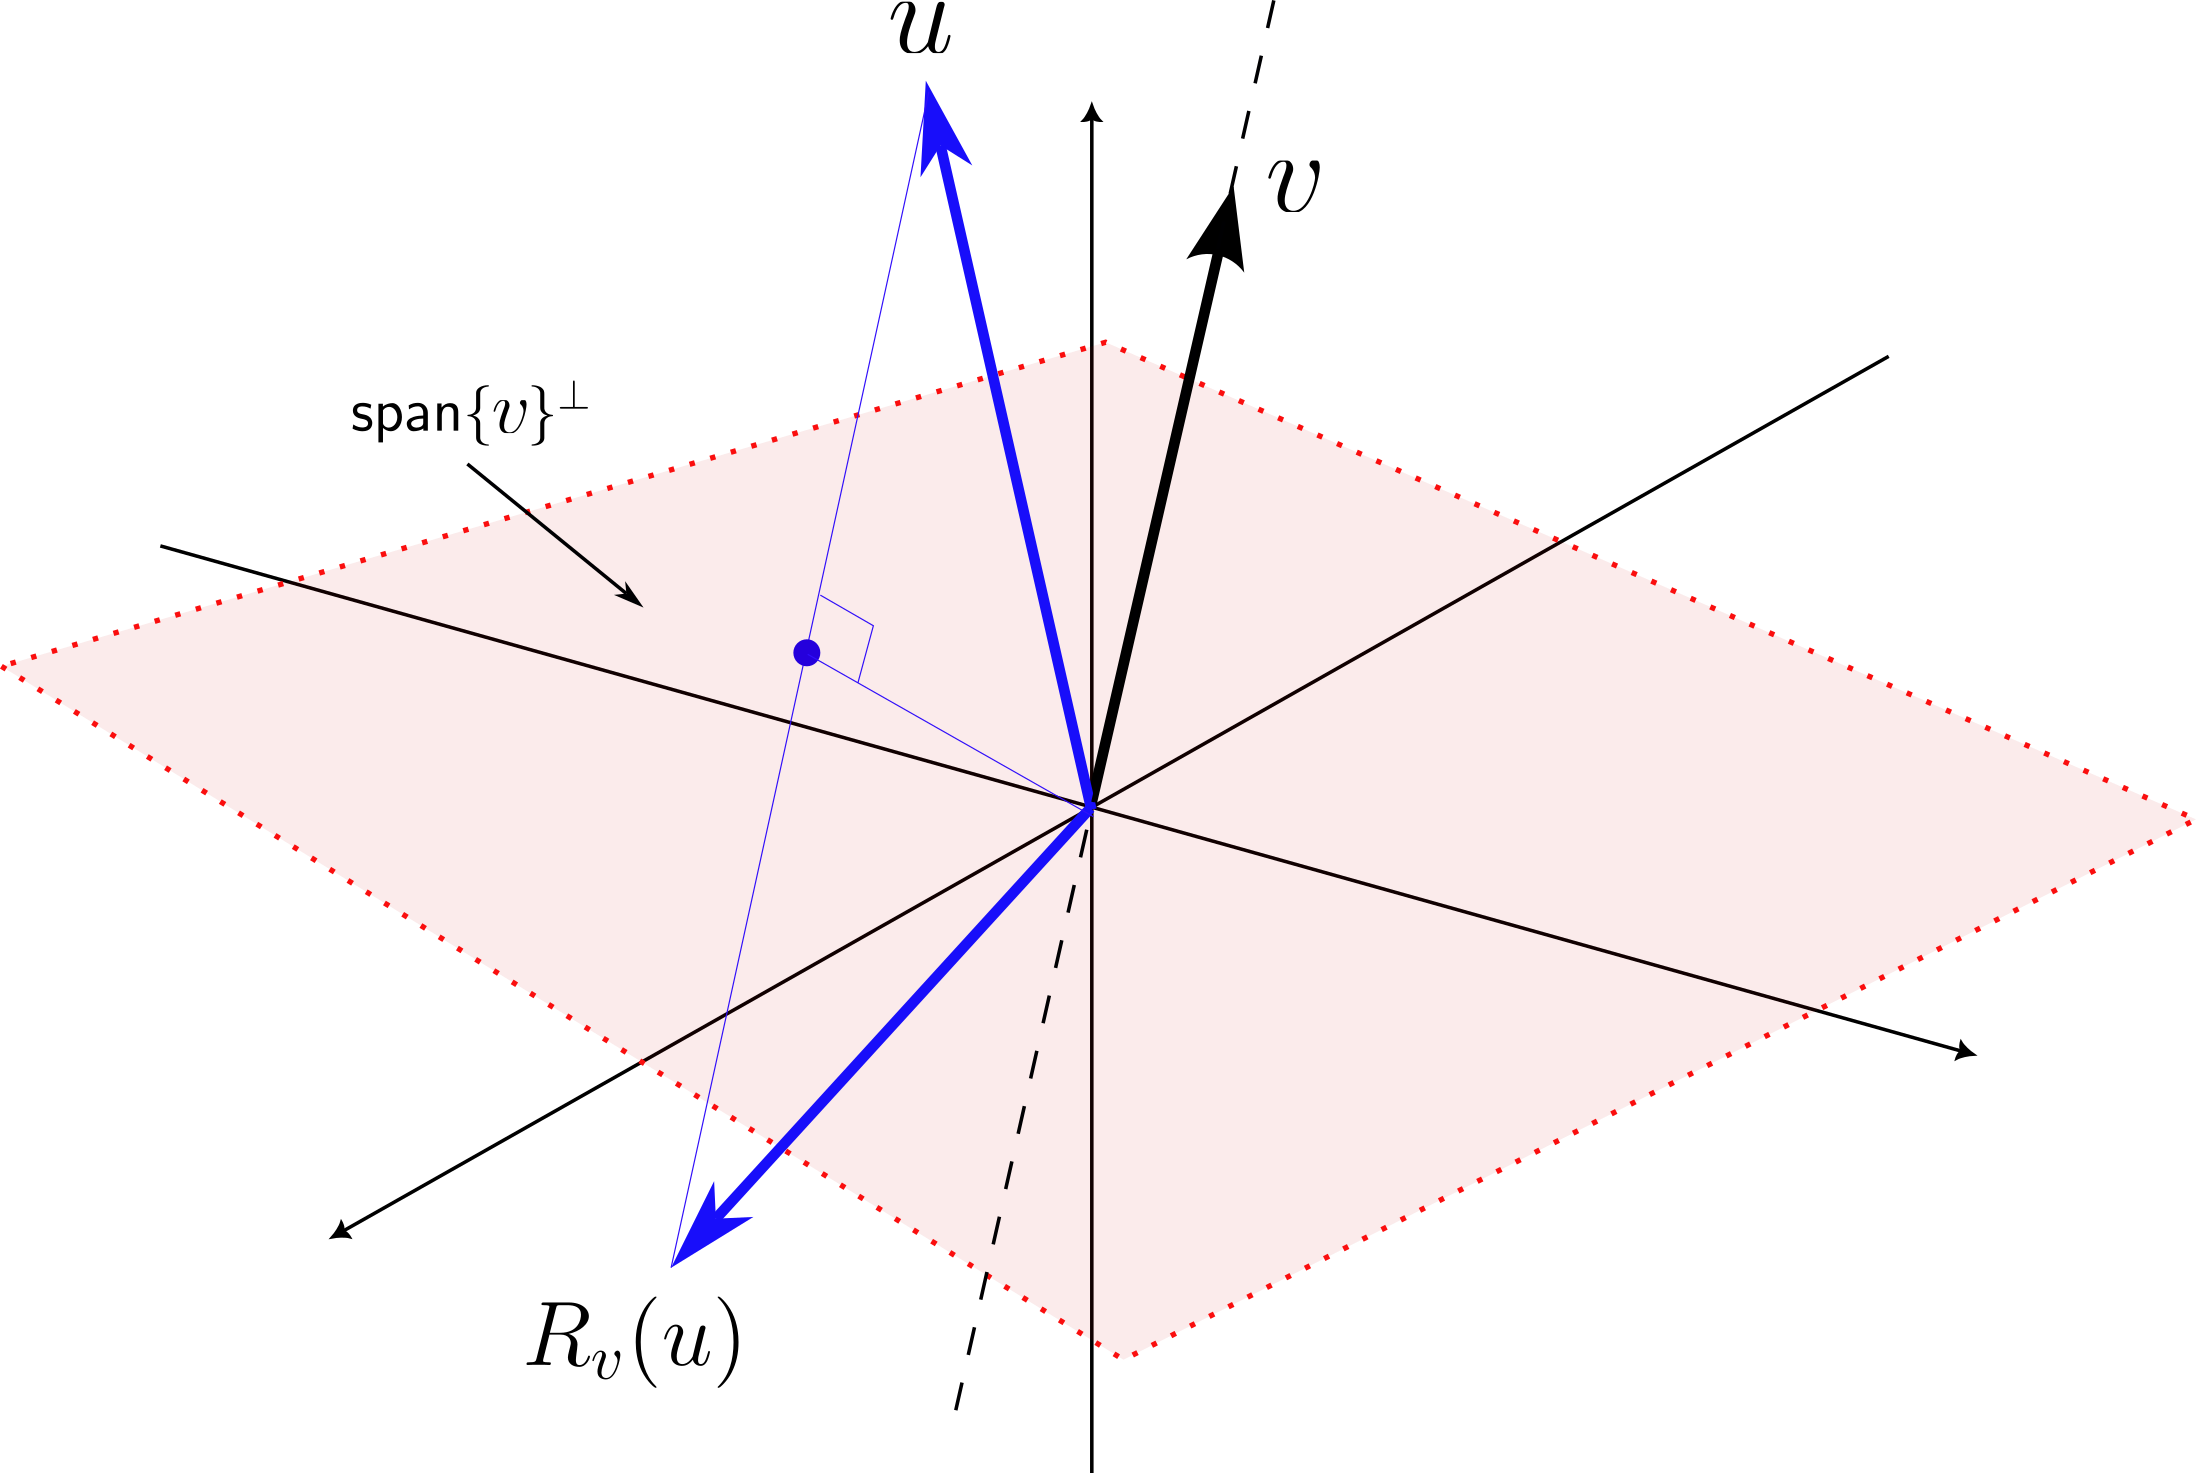
\includegraphics[width=0.6\linewidth]{reflection.png}
    \caption{Diagram of a reflection in $\RR^3$ using the standard inner product.}
    \label{fig:reflectionr3}
\end{figure}
\begin{remark*}
    Let $e_1=v$ and let $e_2,...,e_n$ be a basis for $\Span\{e_1\}^\perp$. Then $B = \{e_1,...,e_n\}$ is a basis for $V$ and $[R]_B = \diag(-1,1,...,1)$. So $\det R_v = -1$. 
\end{remark*}
\begin{defn}
    Let $T : V \to V$ be an isometry. Recall that since $T$ is an isomorphism, $\det T \neq 0$. We say that $T$ is \textbf{proper} if $\det T >0$ and \textbf{improper} if $\det T<0$. \index{Isometry!Proper/Improper}
\end{defn}
\begin{remark*}
    Reflections are improper isometries.
\end{remark*}
\begin{lemma}
    Let $P$ be an isometry. Then $P R_v P^{-1}$ is a reflection, and in fact $P R_v P^{-1} = R_{Pv}$.
\end{lemma}
\begin{proof}
    \begin{align*}
        P R_v P^{-1}(u) &= P(P^{-1}(u) - \frac{2G(P^{-1}(u),v)v}{Q(v)})\\
        &= u-\frac{2 G(P^{-1}(u),P^{-1}(P(v))}{Q(P(v))}P(v)\\
        &= u-\frac{2 G(u,P(v)}{Q(P(v))}P(v)\\
        &= R_{P(v)}(u)
    \end{align*}
    Where we have used the fact that $P$ is an isometry to say $Q(P(v))=Q(v)$ and $G(P^{-1}(x),P^{-1}(y))=G(x,y)$.
\end{proof}
\begin{defn}[$T$-invariant Subspace] Let $T:V\to V$ be linear and let $U$ be a subspace of $V$. We say $U$ is $T$-invariant if $T(U) \subseteq U$.
\end{defn}
\begin{lemma}
    Let $U$ be a $T$-invariant subspace. Then $U^\perp$ is a $T^\dagger$-invariant subspace.
\end{lemma}
\begin{proof}
    Let $v \in U^\perp$. This means that $G(u,v) = 0$ for all $u \in U$. Therefore $G(u,T^\dagger(v))=G(T(u),v) = 0$ for all $v$ since, because $U$ is $T$-invariant, we know $T(u)\in U$. In other words, we have $G(u,T^\dagger(v))=0$ for all $u\in U$, which means by definition that $T^\dagger(v) \in U^\perp$.
\end{proof}
\begin{cor}
Let $T \in \Orth(V,G)$. If $T(U)\subseteq U$, then $T(U^\perp) = U^\perp$.
\end{cor}
\begin{proof}
    We know $T(U)\subseteq U$. Since $T$ is injective, $\dim T(U) = \dim U$. Therefore $T(U)=U$ and $U=T^{-1}(U)$. Therefore $T^\dagger(U)=U$. Applying the lemma, we have $(T^\dagger)^\dagger (U^\perp) \subseteq U^\perp$, so $T(U^\perp)\subseteq U^\perp$, and because $T$ is injective, we furthermore have $T(U^\perp) = U^\perp$.
\end{proof}
\begin{remark*}
    Note that we have not said anything about whether $G|_U$ is nondegenerate or not.
\end{remark*}
\begin{defn}
    We say $V$ is an \textbf{orthogonal direct sum} of the subspaces $U_1,...,U_k\subseteq V$ if $V = \bigoplus_{i=1}^k U_i$ and $U_i\perp U_j$ for all $i\neq j$. Notationally we write $V = U_1 \orthoplus U_2 \orthoplus...\orthoplus U_k = \bigorthoplus_{i=1}^k U_i$.
\end{defn}
\begin{remark*}
    The above definition is about decomposing a vector space into a direct sum of smaller, mutually orthogonal vector spaces. 
\end{remark*}
\begin{remark*}
    Notice that for each $j$, we have $U_j^\perp = \bigoplus_{i=1, i\neq j}^k U_i$.
\end{remark*}
\begin{remark*}
    Suppose that $V = \bigorthoplus_{i=1}^k U_i$, which means that any vector $v$ can be written as $v=\sum_{i=1}^k u_i$, where $G(u_i,u_j) = 0$ if $i\neq j$. Then $Q(v) = \sum_{i=1}^k Q(u_i)$.
\end{remark*}
\begin{lemma}
    Suppose that $V = \bigorthoplus_{i=1}^k \tilde{U}_i$, and $V = \bigorthoplus_{i=1}^k U_i$, and let $v = \sum_{i=1}^k u_i$ and $v = \sum_{i=1}^k\tilde{u}_i$. Suppose for each $i=1,...,k$ we have an isometry $P_i : U_i \to \tilde{U}_i$. Define $P : V \to V$ by $P(\sum_{i=1}^k u_i) = \sum_{i=1}^k P_i u_i$. Then $P$ is an isometry.\label{lemma74}
\end{lemma}
\begin{remark*}
     \begin{align*}Q(P(v)) &= Q(\sum_{i=1}^k P_i(v_i)) \\&= \sum_{i=1}^k Q(P_i(v_i)) \\&= \sum_{i=1}^k Q(v_i) \\&= Q(v)\end{align*}
\end{remark*}
So we can build isometries of $V$ out of isometries on the orthogonal components of $V$.
\subsubsection{Hyperbolic Planes}
We will take a detour here to talk about hyperbolic planes.
\begin{defn}
    Let $U$ be a vector subspace of $V$. Then $U$ is said to be isotropic if $Q|_U=0$, or equivalently $U \subseteq U^\perp$.\index{Isotropic!Subspace}
\end{defn}
\begin{remark*}
    An isotropic vector generates an isotropic vector subspace. That is, if $v$ is isotropic then $\Span\{v\}$ is an isotropic subspace.
\end{remark*}
If $\FF = \RR$ and $G$ is positive definite or negative definite then there are no isotropic subspaces.
\begin{defn}\index{Hyperbolic Plane}
    Let $G$ be a metric on $V$. We say that $V$ is a \textbf{hyperbolic plane} if $\dim V = 2$ and $V$ contains an isotropic vector.
\end{defn}
\begin{thm}
    Let $\dim V = 2$, and let $G$ be a metric. The following are equivalent.
    \begin{enumerate}[i)]
    \item {
    $V$ is a hyperbolic plane.
    }
    \item {
    There exists a basis $B=\{u,v\}$ of $V$ so that $Q(u)=0$, $Q(v)=0$, and $G(u,v)=G(v,u)=1$. That is,
    \[[G]_B = \m{0&1\\1&0}\]
    Such a basis is called a \textbf{hyperbolic basis}\index{Basis!Hyperbolic}
    }
    \item {
    For all bases $B$ of $V$, $\det [G]_B = -x^2$ for some $x \in \FF$.
    }
    \end{enumerate}
\end{thm}
\begin{proof}
    First we show that i implies ii. First, there exists $u$ so that $Q(u)=0$. Then by nondegeneracy there is some $v$ so that $G(u,v)\neq 0$. Then since $G(u,u)=0$, $v\neq u$, so $\{u,v\}$ is a linearly independent set and hence a basis. Without loss of generality we may set $G(u,v)=1$ by rescaling $v$. Then let $a \in \FF$, and set $\tilde{v} = v+au$. Then $Q(\tilde{v}) = Q(v)+2a$. Choose $a = -\frac{1}{2}Q(v)$. So $Q(\tilde{v})=0$ and $\{u,\tilde{v}\}$ is linearly independent, and therefore is a basis satisfying the requirements of ii.

    Now we show that ii implies iii. Let $B$ be the aforementioned basis. Then 
    \[[G]_B = \m{0&1\\1&0}\]
    which has determinant $-1$ as required. If $\tilde{B}$ is another basis then $[G]_{\tilde{B}} = -\det(P_{B\tilde{B}})^2$ which is of the form $-x^2$ as required.

    Finally we show that iii implies i. Suppose $\det [G]_B = -x^2,x\neq0$ for all bases $B$. This means $G$ is nondegenerate, and furthermore there exists a basis $B=\{e_1,e_2\}$ so that $[G]_B = \diag(b_1,b_2)$. This means $b_1b_2 = -x^2$ for some $x$. Now let $w = c_1 e_1 + c_2 e_2$. Then \[Q(w) = c_1^2 b_1 + c_2^2 b_2\]
    Then let $c_1 = a$ and $c_2 = b_2$, so then 
    \[Q(w) = a^2 b_1 + b_1^2 b_2 = b_1(a^2+b_1b_2)=b_1(a^2-a^2)=0\]
    So $w$ is an isotropic vector, which is what we needed to find. This completes the proof.
\end{proof}
\begin{cor}
    Any two hyperbolic planes are isometric.
\end{cor}
\begin{proof}
    Let $V,G$ and $\tilde{V},\tilde{G}$ be two hyperbolic planes. Then there are bases $B=\{e_1,e_2\},\tilde{B}=\{\tilde{e}_1,\tilde{e}_2\}$ so that \[[G]_B = [\tilde{G}]_{\tilde{B}} = \m{0&1\\1&0}\]
    Let $P : V\to \tilde{V}$ so that $P(e_1)=\tilde{e}_1,P(e_2)=\tilde{e}_2$, and extend the definition by linearity. Then $P^T [G]_B P = [G]_{\tilde{B}}$ which means $P$ is an isometry as required.
\end{proof}
\begin{thm}
    Any hyperbolic plane $V$ contains exactly two one-dimensional isotropic subspaces.
\end{thm}
\begin{proof}
    Let $\{u,v\}=B$ be a hyperbolic basis for $V$. Then let $w \in V$. Then $w = au+bv$ and $Q(w)=2ab$. This is zero iff $a=0$ or $b=0$. Therefore $w=au$ or $w=bv$. Thus $w$ is isotropic iff $w \in \Span\{u\}$ or $w\in \Span\{v\}$. These are the two isotropic subspaces.
\end{proof}
\begin{remark*}
    The figure presented earlier, figure \ref{fig:quadform}, shows the isotropic subspaces for the choice of metric,
    \[[G]_S = \m{0&1\\1&0}\]
    Any hyperbolic plane metric can be put in this form, if we use the basis $e_1 = \frac{u+v}{4G(u,v)}$ and $e_2 = \frac{u-v}{4G(u,v)}$. Therefore, figure \ref{fig:quadform} provides a decent visual of what the isotropic subspaces look like. In general, we get the same picture but warped by some shear/rotation.
\end{remark*}
\begin{defn}
    Let $\FF$ be a field. The \textbf{group of units} of $\FF$ is the set of all invertible elements of $\FF$. That is, 
    \begin{equation}\FF^* = \{a \in \FF: \exists b \in \FF, ba=ab=1\}.\end{equation}\index{Group!of Units}
\end{defn}
\begin{thm}
    Let $V,G$ be a hyperbolic plane. Then,
    \begin{enumerate}[a)]
    \item {
    Any improper isometry is a reflection.
    }
    \item {
    The special orthogonal group of $G$ is isomorphic to the group of units of $\FF$. That is, $\SO(V,G) = \FF^*$
    }
    \end{enumerate}
\end{thm}
\begin{proof}
    Let $P\in \Orth(V,G)$ be any orthogonal transformation and let $\{u,v\}$ be a hyperbolic basis. Then $P$ maps isotropic subspaces to isotropic subspaces since $Q(P(v))=Q(v)$. So either $P$ takes $\Span\{u\}$ to $\Span\{u\}$ and $\Span\{v\}$ to $\Span\{v\}$ or it exchanges them. In the first case, $P(u) = au$ and $P(v) = bv$ for some $a,b\in\FF$. Therefore $[P]_B = \diag(a,b)$. So $1=G(u,v)=G(P(u),P(v)) = G(u,v)ab=ab$. Therefore $b=a^{-1}$, meaning $[P]_B = \diag(a,a^{-1})$ and $\det [P]_B = 1$. So $P\in \SO(V,G)$. Therefore every isometry which leaves the two isotropic vector spaces where they are is an element of $\SO(V,G)$.

    In the other case, we have $P(u)=av$ and $P(v)=bu$. So $G(u,v)=ab$, and \[[P]_B = \m{0&a^{-1}\\a&0}\]
    so $\det [P]_B = -1$. This is not an element of $\SO(V,G)$, but it is a reflection. Observe that $P(u+av) = av+a a^{-1}u = u+av$ and $P(u-av) = av-u = -(u-av)$. Since $G(u+av,u-av) = 0+a-a+0=0$, we finally have $P = R_{u-av}$. This proves part a).

    The previous two points imply that $\SO(V,G)$ consists entirely of isometries which leave the two isotropic subspaces where they are.

    Finally, let $\varphi : \SO(V,G) \to \FF^*$ be defined by $\varphi(P) = \varphi(\diag(a,a^{-1})) = a$. This is well defined because we just showed that the only elements of $\SO(V,G)$ are those which can be put in the form $\diag(a,a^{-1})$. This is a group isomorphism since $\varphi^{-1}(a) = \diag(a,a^{-1})$ is defined and 
    \begin{align*}\varphi(AB) &= \varphi(\diag(a,a^{-1})\diag(b,b^{-1})) \\&= \varphi(\diag(ab,(ab)^{-1})) = ab \\&= \varphi(A)\varphi(B)\end{align*}
\end{proof}

\subsubsection{Witt's Cancellation Theorem}
\begin{defn}
   Let $U$ be a subspace of $V$, and let $G$ be nondegenerate. If $G|_U$ is nondegenerate we say $U$ is a \textbf{nondegenerate subspace}.\index{Subspace!Nondegenerate}
\end{defn}
\begin{thm}[Witt Cancellation Theorem]\index{Theorem!Witt Cancellation Theorem}\index{Witt!Cancellation Theorem}
Let $V,G$ be a vector space over a field $\FF$ of characteristic zero where $G$ is a metric. Suppose $U_1,U_2$ are nondegenerate subspaces of $V$. If $U_1$ is isometric to $U_2$ then $U_1^\perp$ is isometric to $U_2^\perp$.\label{thm:wittcancel}
\end{thm}
\begin{proof}
    If $U_1,U_2$ are nondegenerate subspaces then $V = U_1\orthoplus U_1^\perp$ and $V=U_2\orthoplus U_2^\perp$. So what we are trying to show is that if $U_1$ and $U_2$ are isometric, we can ``cancel" them on both sides of the equation $U_1\orthoplus U_1^\perp = U_2\oplus U_2^\perp$.

    First observe that $G|_{U_1}$ and $G|_{U_2}$ are both nondegenerate.

    Now, let $U_1$ and $U_2$ be isometric. Then first of all, $\dim U_1 = \dim U_2 = k$. We will prove this by using mathematical induction on $k$. Let us begin with $k=1$ as the base case.

    In the base case, $U_1 = \Span\{u_1\}$, $U_2=\Span\{u_2\}$, and $Q(u_1)\neq 0, Q(u_2)\neq 0$. By scaling $u_2$ appropriately, let $Q(u_1)=Q(u_2)$. Then \[Q(u_1\pm u_2) = Q(u_1)\pm 2G(u_1,u_2)+Q(u_2) = 2Q(u_1)\pm 2G(u_1,u_2)\]
    
    We claim that either $Q(u_1+u_2)\neq 0$ or $Q(u_1-u_2)\neq 0$ (but not both!)

    If they are both zero, then we could expand then add them together and get $Q(u_1)=Q(u_2)=0$.

    If we know that $Q(u_1+u_2)\neq 0$, then we also know that $G(u_1+u_2,u_1-u_2) = Q(u_1)-Q(u_2)=0$, so $u_1+u_2\perp u_1-u_2$. Furthermore, $R_{u_1+u_2} (u_1-u_2)=u_1-u_2$, and so \[R_{u_1+u_2}(u_1-u_2)+R_{u_1+u_2}(u_1+u_2) = R_{u_1+u_2}(2u_1) = -2u_2\] This means that $R_{u_1+u_2}$ takes $\Span\{u_1\}$ to $\Span\{u_2\}$ and vice versa, and also that $R_{u_1+u_2}$ takes $\Span \{u_1\}^\perp$ to $\Span\{u_2\}^\perp$. Therefore $R_{u_1+u_2}$ is an isometry between $U_1^\perp$ and $U_2^\perp$ as required.

    Now suppose instead that we know $Q(u_1-u_2)\neq 0$. Then we could take $R_{u_1-u_2}$ and find $R_{u_1-u_2}(u_1)=u_2$, and then get the same result. This finishes the base case.

    See Jacobson chapter 6 for the inductive step \cite{Jacobson2009-pp}. 
\end{proof}
\begin{remark*}
    Witt's Cancellation theorem, along with lemma \ref{lemma74} hints at the fact that if we have an isometry between nondegenerate subspaces $U_1$ and $U_2$, then we can extend it to an isometry from $V$ to $V$. This will be proven at the beginning of next lecture.
\end{remark*}
\subsection{Lecture 8: Witt Extension Theorem, Maximally Isotropic Subspaces, and the Cartan-Dieudonn\'e Theorem}
\subsubsection{Witt Extension Theorem}
\begin{lemma}
    Let $V,G$ be a vector space with metric, and let $U\subseteq V$ be a degenerate subspace. That is, a subspace with $\Radical (G|_U) \neq \{0\}$. Let $U'$ be any subspace with the property that $V=U' \oplus \Radical(G|_U)$. Let $r = \dim \Radical(G|_U)$. Then there exist hyperbolic planes $H_1,...,H_r$ and a subspace $W \subseteq V$ so that $U\oplus W = U'\orthoplus H_1\orthoplus ...\orthoplus H_r$.
\end{lemma}
\begin{remark*}
    This lemma says that if we have a degenerate subspace $U$, there is always some other subspace $W$ we can add it to and get a nondegenerate subspace. Furthermore, the sum of these two subspaces decomposes into a nice nondegenerate space $U'$ along with a bunch of hyperbolic planes $H_i$, which are easy to work with.
\end{remark*}
\begin{proof}
    Let $\{u_1,...,u_r\}$ be a basis of $\Radical(G|_U)$. Let $\alpha \in U^*$ be defined so that $\alpha(u_1)=1$ and $\alpha(u_i)=0$ for $i=2,...,r$ and $\alpha(U')=0$. 
    
    Then since $G$ is nondegenerate on $V$ there exists some $v_1 \in V$ so that $\alpha(u)=G(u,v_1)$ for all $u$. So, there is some $v_1$ with $G(u_1,v_1)=1$, $G(u_i,v_1)=0$ for $i=2,...,r$, and $G(u,v_1)=0$ for all $u\in U'$. 
    
    Note that $v_1$ is not an element of $U$. Then replace $v$ by $\tilde{v}_1 = v_1+\sigma u_1$, for some $\sigma \in \FF$. 
    
    Then $Q(\tilde{v}_1) = Q(v_1)+2\sigma$. So we set $\sigma = -Q(v_1)/2$, to get $\{u_1,\tilde{v}_1\}$ to span a hyperbolic plane. So we set 
    $H_1 = \Span\{u_1,\tilde{v}_1\}$.
    
    Furthermore, by definition of $\perp$ we have $V = H_1\orthoplus H_1^\perp$. Now let $\tilde{U} = U' \oplus \Span\{u_2,...,u_r\}\subseteq \Span\{u_1,v_1\}^\perp$.
    
    Note that $\Radical(G|_{\tilde{U}}) = \Span\{u_2,...,u_r\}$. If $r=1$ we have $U' = \tilde{U}$ and we can let $W = \Span\{v_1\}$ so that $U\oplus W = U' \oplus H_1$. 
    
    Otherwise, set $U,V = \tilde{U},\tilde{V}$ in the above argument and repeat. Inductively, we will get $r$ hyperbolic planes $H_1,...,H_r$ until finally we have $U\oplus W = U' \orthoplus H_1\orthoplus...\orthoplus H_r$ as required. We also verify that $U\oplus W$ is nondegenerate, since everything in the big orthogonal direct sum is.  
\end{proof}
\begin{remark*}
    This proof is quite inscrutable. The idea is that, since $U$ is degenerate, we can find an isotropic vector $u_1$ in $U$. This vector gives us the first basis vector for the hyperbolic plane. Then we find another vector, $\tilde{v}_1$ which is also isotropic, and the span of the two isotropic vectors gives us the first hyperbolic plane $H_1$. Then, we check whether the complement of $H_1$ in $U$ is degenerate. If not, we are done and $W$ is just the span of $v_1$. Otherwise, since the complement is degenerate we can find another isotropic vector and repeat the process.

    The main idea is to find all of the linearly independent isotropic vectors in $U$, and pair each of them up with an isotropic vector in the larger space $V$ so that their span is non degenerate. To do this, we have to make $U$ into a bigger subspace, which is $U\oplus W$.
\end{remark*}

\begin{thm}[Witt Extension Theorem] Let $U_1$, $U_2$ be subspaces of $V$ and let $P : U_1\to U_2$ be an isometry. Then there exists an isometry $P:V\to V$ so that $P|_{U_1} = \tilde{P}$.\index{Theorem!Witt Extension Theorem}\index{Witt!Extension Theorem}
\end{thm}

\begin{proof}
    If $U_1$ is nondegenerate, this is a direct consequence of Theorem \ref{thm:wittcancel} and Lemma \ref{lemma74}.

    If $U_1$ is degenerate, then there exists some $W_1$ so that $U_1\oplus W_1 = U_1' \orthoplus H_1\orthoplus...\orthoplus H_r$, where $U_1'$ has the property that $U_1 = \Radical(G|_{U_1})\oplus U_1'$. Let $\tilde{P} = P|_{U_1}$. Then $\tilde{P}$ maps $U_1$ to $U_2$, and $\tilde{P}|_{\Radical(G|_{U_1})}$ is an isomorphism between $\Radical(G|_{U_1})$ and $\Radical(G|_{U_2})$. We then set $U_2' = P(U_1')$m which means there exists $W_2$ so that $U_2\oplus W_2 = P(U_1')\orthoplus H_1\orthoplus...\orthoplus H_r = U_2' \orthoplus\tilde{H}_1\orthoplus...\orthoplus \tilde{H}_r$. Here, $H_i = \Span\{v_i,u_i\}$ and $\tilde{H}_i = \Span\{\tilde{v}_i,P(u_i)\}$.

    Now we define $L : U_1\oplus W_1 \to U_2 \oplus W_2$ by $L|_{U_1} = P$ and $L|_{W_1}(v_i) = \tilde{v}_i$ for $i=1,...,r$. Since $v_i \in W_1$, $\tilde{v}_i\in W_2$, and $U_1\oplus W_1$ is nondegenerate, this is an isometry by construction. Since $U_1\oplus W_1$ is nondegenerate, we then see that by Theorem \ref{thm:wittcancel} and Lemma \ref{lemma74}, $L$ can be extended to all of $V$. Since $L$ is in turn an extension of $P$, we are done.
\end{proof}
\begin{remark*}
    A useful application of this theorem is the Witt index.
\end{remark*}
\subsubsection{Maximally Isotropic Subspaces}
\begin{remark*}
    Recall that $U_1$ is an isotropic subspace if $G|_{U_1} = 0$. If $U_2$ is another isotropic with $\dim U_1 = \dim U_2$ then any isomorphism between $U_1$ and $U_2$ is an isometry, and can be extended to $V$ to get an isometry.
\end{remark*}
\begin{defn}[Maximally Isotropic Subspace]\index{Subspace!Maximally Isotropic}
An isotrophic subspace $U\subseteq V$ is said to be \textbf{maximal} if whenever we have another isotropic space $W$ with $U\subseteq W\subseteq V$, then $U=W$.
\end{defn}
\begin{lemma}
    If $U$ is maximally isotropic and $\tilde{U}$ is isotropic then there is an isometry $P : V \to V$ with $P(\tilde{U})\subseteq U$.
\end{lemma}
\begin{proof}
    Suppose $\dim \tilde{U} < \dim U$. Then there is a subspace of $U$ of dimension $\dim \tilde{U}$, and therefore an isomorphism between $\tilde{U}$ and a subspace of $U$. Since any isomorphism between isotropic subspaces is an isometry, this case is done.

    If $\dim \tilde{U} \geq \dim U$, then there is an isometry $P$ with $P(U)\subseteq \tilde{U}$, which means $P^{-1}(\tilde{U})$ is isotropic. This means $U \subseteq P^{-1}(\tilde{U})\subseteq V$. Since $U$ is maximal, $P^{-1}(\tilde{U}) = U$, so $\tilde{U} = P(U)$. This completes the proof for all possible cases.
\end{proof}

\begin{cor}
    All maximally isotropic subspaces of $V$ are the same dimension.
\end{cor}
\begin{proof}
    If $U$ and $\tilde{U}$ are maximally isotropic, then $\dim U \leq \dim \tilde{U}$ by the previous lemma, and vice versa, so $\dim U = \dim \tilde{U}$.
\end{proof}
\begin{defn}[Witt Index]\index{Witt!Index}
    Let $U$ be a maximally isotropic subspace. Then we define $\nu(V) = \dim U$ to be the \textbf{Witt index} of $V$. Notice that it does not depend on the choice of maximally isotropic subspace.
\end{defn}

\begin{lemma}
    Let $\dim V = n$. Then $\nu(V) \leq \floor{\frac{n}{2}}$.\label{lemma83}
\end{lemma}
\begin{proof}
    Let $U$ be a maximally isotropic subspace of $V$. Then $U$ can be extended into $U\oplus W = \bigoplus_{i=1}^r{}_\perp H_i$, where $U' = \{0\}$ since $U$ is maximally isotropic. Since $\dim H_i = 2$, we have $\dim U\oplus W = \nu(V) + \dim W = 2r\leq  n$. So $r \leq \frac{n}{2}$. Since $r$ is an integer, we furthermore have $r\leq \floor{\frac{n}{2}}$. Since $U$ is isotropic, $\Radical (G|_{U}) = U$, so $r=\dim U$. This completes the proof.
\end{proof}
\begin{defn}[Anisotropic Kernel]
    Let $U$ be maximally isotropic. Then there is some $W$ so that $U\oplus W$ is nondegenerate and $V = (U\oplus W)\orthoplus(U\oplus W)^\perp$, where $(U\oplus W)^\perp$ is anisotropic. The space $(U\oplus W)^\perp$ is called an \textbf{anisotropic kernel} of $G$.
\end{defn}
\begin{remark*}
    Let $\mu \leq \nu$. Suppose we had the following decompositions of $V$, where $X$ and $\tilde{X}$ are anisotropic subspaces,
    \[V = H_1\orthoplus...\orthoplus H_\nu \oplus X\]
    \[V = \tilde{H}_1\orthoplus...\orthoplus \tilde{H}_\nu \oplus \tilde{X}\]
    Let $\{\tilde{u}_i,\tilde{v}_i\}$ be a hyperbolic basis for $\tilde{H}_i$ for each $i=1,...,\nu$. Then $\Span\{\tilde{u}_1,...,\tilde{u}_\mu\}$ is isotropic, and $\mu \leq \nu$, so there is an isometry between $H_1\orthoplus...\orthoplus H_\mu$ and $\tilde{H}_1\orthoplus...\orthoplus \tilde{H}_\mu$. By the extension theorem we can extend this to an isometry $H_{\mu+1}\orthoplus...\orthoplus H_\nu \orthoplus X \to\tilde{X}$. But $\tilde{X}$ is anisotropic, so $\mu=\nu$ and $\tilde{X}=X$. So the study of metrics reduces up to isometry to the study of anisotropic metric vector spaces. For general $\FF$ this becomes complicated.
\end{remark*}
    \subsubsection{Classification of Bilinear Forms: Symmetric Bilinear Forms Part 4, Cartan-Dieudonn\'e theorem}
    \begin{thm}[Cartan-Dieudonn\'e Theorem]
    Let $\FF$ be a field of characteristic not equal to $2$. Let $G$ be a metric on $V$, and let $\dim V = n$. Let $P$ be an isometry of $V$. Then $P$ is the product of $k\leq n$ reflections.\index{Theorem!Cartan-Dieudonn\'e Theorem}\end{thm}
    \begin{proof}
        We prove this by induction on $n$.
        
        First suppose $n=1$ for the base case.
        Let $\{v\}$ be a basis of $V$. Then $Pv =\lambda v$ for some $\lambda$, so $Q(P(v))=\lambda^2 Q(v)$. So $\lambda = \pm 11$. In the positive case $P=\One$ and in the negative case $P = R_{-v}$. So $P$ is either a product of zero or one reflections as required.

    The inductive step splits into three cases.
    \begin{enumerate}
    \item {
    Let $V_1 = \{v\in V :Pv = v\}$. Suppose $V_1$ is anisotropic. Then there exists $u\neq 0$ so that $Q(u)\neq 0$ and $P(u) = u$. So $P$ maps $\Span\{u\}^\perp$ to $\Span\{u\}^\perp$, and so $P|_{\Span\{u\}} = \One$, so $P = \One_{1\times 1} \oplus P|_{\Span\{u\}^\perp}$. So the problem reduces to $\Span\{u\}^\perp$ which is $n-1$ dimensional. If it is anisotropic, we repeat the procedure. Otherwise we go to another one of the cases, and try to show that $P|_{\Span\{v\}^\perp}$ and hence $P$ is the product of at most $n-1$ reflections.
    }
    \item {
    Suppose there exists $u\neq 0$ so that $Q(v)\neq 0$ and $Q(v-P(v))\neq 0$. Since $P$ is an isometry, $Q(P(v))=Q(u)\neq 0$. So \begin{align*}R_{v-P(v)}(v+P(v)) &= v+P(v) - \frac{G(v+P(v),v-P(v))(v-P(v))}{Q(v-P(v))} \\&= v+P(v) - \frac{Q(v)-Q(P(v))}{Q(v-P(v))}(v-P(v)) \\&= v+P(v)\end{align*}
    Similarly, $R_{v-P(v)}(v-P(v))=-(v-P(v))$. From this, we see that 
    \begin{align*}
        R_{v-P(v)}(P(v)) &= \frac{1}{2}R_{v-P(v)}(P(v)-v + P(v)+v)\\
        &= \frac{1}{2}(v-P(v)) + \frac{1}{2}(v+P(v))\\
        &= v
    \end{align*}
    This means $R_{v-P(v)}\circ P|_{\Span\{v\}} = \One$. So $P = \One_{1\times 1} \oplus P|_{\Span\{v\}^\perp}$. By induction, we see if we can find $v$ satisfying the original condition but on $\Span\{v\}^\perp$. In general the problem reduces to $\Span\{v\}^\perp$ which is $n-1$ dimensional, so we try to show that $P|_{\Span\{v\}^\perp}$ and hence $P$ is the product of at most $n-1$ reflections
    }
    \item {
    If $V$ is anisotropic then suppose there exists a vector $v \in V_1$ as above. Then case 1 holds. Suppose $V$ is anisotropic and $V_1$ is empty, then for any vector $v\neq 0$ we have $v-P(v)\neq 0$, so $Q(v)\neq 0$ and $Q(v-P(v))\neq 0$. Then case 2 holds. Finally, we come to the last case. Suppose $V$ is not anisotropic, and there exists $u \neq 0$ so that $Q(u)=0$. Then we have two sub-cases, $n=2$ and $n>2$.
    \begin{enumerate}[i)]
    \item {
    $n=2$. If $n=2$ and $V$ has an isotropic vector, then $V$ must be a hyperbolic plane. Let $\{u,v\}$ be a hyperbolic basis. Then $P$ is an isometry, we have $P : u \mapsto au$ and $P : v \mapsto bv$ or $P:u\mapsto av$ and $P:v\mapsto bu$. Consider the first one, where $P$ is diagonal. If $a=1$ then $P$ is just the identity. Otherwise, assume $a\neq 1$ and let $w=u+v$. Then $w-P(w) = u+v-au-a^{-1}v \neq 0$, so $Q(w) = 2$ and $Q(w-P(w))=2(1-a)(1-a^{-1})$. So case 2 holds. Now suppose $P$ swaps $u$ and $v$. Then $P=R_{u-av}$. Therefore we are done.
}
\item {
Assume $n\geq 3$. Assume $V_1 = \ker(\One-P)$ is not anisotropic, and if $Q(v)\neq 0$ then $Q(v-P(v))=0$. The claim is that $Q(u-P(u)) = 0$ for all $u\in V$. Since we have assumed this is true for all anisotropic vectors, it suffices to prove it for all isotropic vectors. First of all, we have $Q(w-P(w)) = Q(P(w)) - 2G(w,P(w))$.

Note that $\Span\{w\}^\perp$ is $n-1$ dimensional, and since $n\geq 3$ we have $n-1\geq \floor{n/2}$. So $\Span\{w\}^\perp$ is not isotropic because if it were, it would violate Lemma \ref{lemma83}. So there must be some $u\in \Span\{w\}^\perp$ with $Q(u)\neq 0$ and $u\neq 0$. Then $G(w\pm u,w) = \pm G(u,w) = 0$. So $w\pm u \in \Span\{w\}^\perp$. So $Q(w\pm u) = Q(u)\neq 0$. Let $L = \One - P$. Then $Q(L(u)) = 0$ for all $u\in V$ as we stated at the beginning, so $Q(L(w\pm u)) =0 $. But then $Q(L(w)+L(u)) = Q(L(w))+2G(L(w),L(u))$ and $Q(L(w)-L(u))=Q(L(w))-2G(L(w),L(u))$. So $Q(L(w)+L(u))+Q(L(w)-L(u)) = 2Q(L(w))=0$. So $Q(w-P(w))=0$ as required.

Since $Q(u-P(u)) =0$ for all $u$, $\image(L)$ is isotropic. From assignment 2 we also have that $\ker (\One-P) = \im (\One-P)^\perp$, so $\image(\One-P)^\perp$ and $\image(1-P)$ are isotropic. So $V_1 \subseteq V_1^\perp$. Since $V_1^\perp$ is isotropic, $V_1^\perp \subseteq V_1$. So $V_1=V_1^\perp$. Hence $\image(\One-P) = \ker(\One-P)$. So $(\One-P)^2=0$. So $\One-P$ is nilpotent. From the Jordan canonical form of $\One-P$ we see that the matrix of $\One-P=L$ in the Jordan basis $J$ will look like all zeros, except for the first upper diagonal line which will be all ones. It follows that $P=\One-L$ will have all $1$'s on the diagonal.
\begin{equation}
[P]_J = 
\m{
1&-1&&&&\\
&1 &-1&&&\\
 &  &1&-1 &&\\
 &&&&\ddots&&\\
 &&&&1&-1\\
 &&&&&1
}
\end{equation}
Where there are zeros everywhere except shown.
So $\det P = 1$, which means $P$ is a proper isometry. In this case we also have $\dim V_1 = \dim V_1^\perp$, so $\dim V = 2\dim V_1$, which means $\dim V$ is even.

This means that any improper isometry meets the criteria of one of the previous cases! So any improper isometry is the product of at most $n-1$ reflections. 

Now let $R_w$ be a reflection and let $\tilde{P}=R_w P$. Since $P$ is proper, $\tilde{P}$ is improper. So $\tilde{P}$ is the product of at most $n-1$ reflections. Since $R_w^{-1} = R_w$, we  see that $P = R_w \tilde{P}$, so $P$ is the product of at most $n$ reflections as required.
}
    \end{enumerate}
    }
    \end{enumerate}
    \end{proof}
\begin{thm}[Classification of Symmetric Bilinear Forms]\index{Theorem!Classification of Symmetric Bilinear Forms}
The classification of symmetric bilinear forms refers to the following theorems
\begin{itemize}
\item {Sylvester's Law of Inertia}
\item {Witt Extension Theorem}
\item {Cartan-Dieudonn\'e Theorem}
\end{itemize}
Together, these three theorems allow one to determine a massive amount of information about a given metric.
\end{thm}

\subsection{Lecture 9: Skew-Symmetric Bilinear Forms and the Pfaffian}
\subsubsection{Classification of Bilinear Forms: Skew-Symmetric Bilinear Forms}
The skew symmetric case is actually a lot easier than the symmetric case. 
\begin{thm}[Classification of Skew-Symmetric Bilinear Forms]\index{Theorem!Classification of Skew-Symmetric Bilinear Forms}
Let $\textsf{char} \FF \neq 2$ and let $V$ be a vector space over $\FF$. Let $G$ be a skew-symmetric bilinear form over $V$. Then there exists a basis $B = \{e_1,f_1,...,e_r,f_r,g_1,...,g_{n-2r}\}$ so that
\begin{enumerate}
\item {$G(e_i,e_j)=0$ for all $i,j$, $G(f_i,f_j)=0$ for all $i,j$, $G(g_i,g_j)=0$ for all $i,j$.}
\item {$G(e_i,f_j)=-G(f_j,e_i)=\delta_{ij}$.}
\item {$G(v,g_\ell)=0$ for all $\ell=1,...,n-2r$.}
\end{enumerate}
In this basis we have,
\begin{equation}
    [G]_B = \m{
    0&1& & & &\\
   -1&0& & &\\
     & &0&1& &\\
     &&-1&0& &\\
     & & & &\ddots &\\
     & & & & &0&1&\\
     & & & &&-1&0&\\
     & & & & & & &0
    }
\end{equation}
Where there are zeros everywhere nothing is shown. In the bottom right corner, note that there is only a zero if $\dim V$ is odd.
\end{thm}
\begin{remark*}
    If $\dim V$ is odd, then $\det [G]_B = 0$. So $\det [G] = 0$ in every basis. So $G$ is degenerate.
\end{remark*}
\begin{cor}
    If $G$ is nondegenerate then $\dim V$ is even.
\end{cor}
\begin{proof}
    If $G=0$ then $r=0$ and we are done. So suppose $G\neq 0$. Then there exist some $e_1,\tilde{f}_1$ so that $G(e_1,\tilde{f}_1)=a\neq 0$. Set $f_1 = \tilde{f}_1/a$. So $G(f_1,e_i)=-1$ and, because $G$ is skew symmetric, this means $B_1=\{e_1,f_1\}$ is linearly independent. Let $V_1 = \Span\{e_1,f_1\}$. Then 
    \[[G|_{V_1}]_{B_1} =\m{0&-1\\1&0}\]
    and $|\det [G|_{V_1}]_{B_1}| =1$, so $V_1$ is nondegenerate. Set $V=V_1\orthoplus V_1^\perp$, then pick any $e_2,\tilde{f}_2 \in V_1^\perp$ satisfying $G(e_2,f_2)=a\in \FF$. Since they are elements of $V_1^\perp$ we also satisfy the other required identities. We keep doing this, and by induction we can find some number $r$ of pairs $\{e_i,f_i\}$ which satisfy $G(e_i,f_i)\neq 0$ and the other identities. Finally, we observe that $V = V_1\orthoplus ...\orthoplus V_r \oplus V^\perp$. So we finally let $\{g_1,...,g_{n-2r}\}$ be a basis for $V^\perp$, and the theorem is complete.
\end{proof}
\begin{remark*}
    Recall that a skew symmetric bilinear form on $V$ is also an element of $\Lambda^2 V^*$. So we have just completely characterized all possible elements of $\Lambda^2 V^*$.
\end{remark*}
\begin{defn}\index{Symplectic Form}\index{Form!Symplectic}
    Let $\dim V = 2k$ be even. A nondegenerate skew-skymmetric bilinear form on $V$ is called a \textbf{symplectic form}. It is usually denoted $\omega$.
\end{defn}
\begin{defn}
    Let $V$ and $W$ be even dimensional vector spaces, and let $G$ and $H$ be symplectic forms on $V$ and $W$ respectively. Then an isomorphism $\phi : V \to W$ with $\phi^* H = G$ is called a \textbf{symplectic isomorphism}, or symplectomorphism. It is the equivalent of an isometry for skew-symmetric bilinear forms.\index{Isomorphism!Symplectic}\index{Symplectomorphism}
\end{defn}
\subsubsection{The Pfaffian}
We've just shown that given any skew-symmetric bilinear form on $V$ there is a basis where either $\det [G]_B = 0$ or $\det [G]_B = 1$. Suppose we choose a different basis $C$. Then let $P_{CB}$ be the change of basis map. We have
\[\det [G]_C = \det(P_{CB})^2 \det [G]_B = \begin{cases}0&n=2k+1\\1&n=2k\end{cases}\]
So for any basis $C$, the value of $\det [G]_C$ is a perfect square in $\FF$. We can use this to construct an invariant of $G$ (that is, a scalar function of $G$ which is invariant under isometries of $G$).
\begin{cor}
    Any two skew-symmetric matrices $A$ and $B$ are related by a change of basis transformation $P^T B P = A$ if and only if $\rank A = \rank B$.
\end{cor}
\begin{proof}
    Suppose $\rank A = \rank B$. Then the dimension of $V^{\perp_A}$ is the same as the dimension of $V^{\perp_B}$ by definition. Therefore both matrices can be put into the same canonical form, which by transitivity means they are related by a change of basis transformation.
    
    The converse holds due to the fact that $\rank$ is already known to be an invariant of bilinear forms, so $\rank A = \rank P^T B P = \rank B$.
\end{proof}

\begin{example}
Some examples.
    \begin{enumerate}[i)]
    \item {Let $n=3$. Then 
    \[A = \m{0&a&b\\-a&0&c\\-b&-c&0},\qquad \det A = 0\]
    }
    \item {Let $n=2$. Then
    \[A = \m{0&a\\-a&0},\qquad \det A = a^2\]
    }
    \end{enumerate}
\end{example}

Let $\{x_{ij}:i,j=1,...,n\}$ be some variables (it does not matter what set they take values in, we are just using them symbolically).
\begin{defn}
Consider the set of all polynomials, whose variables are $\{x_{ij}\}$ and whose coefficients are in $\ZZ$. We will call this set $\ZZ[x_{ij}]$.\index{Ring!of Polynomials}
\end{defn}
\begin{remark*}
Some remarks are as follows.
    \begin{enumerate}
    \item {The only elements $f\in \ZZ[x_{ij}]$ with $f^{-1}\in \ZZ[x_{ij}]$ are $f=\pm 1$.}
    \item {
    The set $\ZZ[x_{ij}]$ forms a \textbf{ring} with respect to multiplication and addition.
    }
    \item {
    If $f\neq 0,g \neq 0$ then $fg\neq 0$. So the ring $\ZZ[x_{ij}]$ is an \textbf{integral domain}.\index{Integral Domain}
    }
    \item {The ring $\ZZ[x_{ij}]$ is a \textbf{unique factorization domain}\index{Unique Factorization Domain}. For any $f \in \ZZ[x_{ij}]$ there is a unique set of polynomials $g_1,...,g_r \in \ZZ[x_{ij}]$ so that $f = \pm g_1...g_r$.
    }
    \end{enumerate}
\end{remark*}
\begin{defn}
    Let $\QQ(x_{ij})$ denote the \textbf{field of fractions} of $\ZZ[x_{ij}]$. That is, all rational functions $f/g$ where $f$ and $g$ are polynomials with integer coefficients.\index{Field!of Fractions of Polynomial Ring}
\end{defn}
\begin{remark*}
    We are about to use the fact that $x_{ij} \in \QQ(x_{ij})$ and $-x_{ij} \in \QQ(x_{ij})$.
\end{remark*}
\begin{lemma}
    Let $X$ be the matrix formed by setting $X_{ii}=0$ for all $i=1,...,n$, $X_{ij}=x_{ij}$ for all $i<j$, and $X_{ij}=-x_{ij}$ for all $i>j$. Then there exist integer polynomials $f,g$ so that $\det X = f^2/g^2$.
\end{lemma}
\begin{proof}
    Since $X$ is a skew symmetric matrix and $\FF = \QQ(x_{ij})$ is a field, we know that $\det X$ is a perfect square in $\FF$.
\end{proof}
\begin{remark*}
    Without loss of generality, $f^2$ and $g^2$ share no common factors in $\FF$. But since $\FF$ is a field, $f^2\in\FF$ is automatically divisible by $g^2\in \FF$. Therefore it is sufficient to take $g = \pm 1$, so $g^2 = 1$. Thus we have $\det X = f^2$ for some $f \in \ZZ[x_{ij}]$. This means that $f$ is determined up to a sign by the formula $\det X = f^2$. We can use this to define the Pfaffian for any commutative ring $R$ with $1+1\neq 0$.
\end{remark*}
\begin{remark*}
    Given a ring $R$, there is a unique ring homomorphism from $\ZZ[x_{ij}]$ to $R$, which takes each monomial $x_{ij}$ to some element of $R$. That is, there exists $\phi : \ZZ[x_{ij}]\to R$ with $\phi(x_{ij}) = A_{ij}$ for each $i,j$ and so that $\phi(h(x_{11},...)) = h(\phi(x_{11}),...)$. This is similar to extending a definition by linearity, excep we are extending it as a ring homomorphism instead.
\end{remark*}
\begin{remark*}
    Let $A_0$ denote the standard matrix,
    \[    A_0 = \m{
    0&1& & & \\
   -1&0& & \\
     & &0&1& \\
     &&-1&0& \\
     & & & &\ddots \\
     & & & & &0&1\\
     & & & &&-1&0\\
    }\]
    Then $f(A_0) = \pm 1$, since $\det A_0 = 1$. 
\end{remark*}
\begin{defn}[Pfaffian]
Let $R$ be a commutative ring with $1+1\neq 0$ and let $\textsf{Skew}(M_{nn}(R))$. Then we define the Pfaffian to be the unique function $\Pf : \textsf{Skew}(M_{nn}(R))\to R$ with $\Pf(A_0) = 1$ and $\Pf(A)^2 = \det A$ for all skew symmetric $A$.
\end{defn}
\begin{example}
Some examples.
    \begin{enumerate}
    \item {When $n=2$, we have
    \[\Pf\m{0&a\\-a&0} = a\]
    }
    \item {
    When $n=4$ we have,
    \[\Pf\m{0&A_{12}&A_{13}&A_{14}\\
    -A_{12}&0&A_{23}&A_{24}\\
    -A_{13}&-A_{23}&0&A_{34}\\
    -A_{14}&-A_{24}&-A_{34}&0} = A_{12}A_{34}-A_{13}A_{24}+A_{14}A_{23}
    \]
    }
    \end{enumerate}
\end{example}
\begin{thm}
    Let $\omega$ be a skew-symmetric bilinear form. Then $\Pf(\omega)$ is well defined, and is invariant with respect to isometries.\index{Invariant!Pfaffian of Skew-Symmetric Bilinear Form}
\end{thm}
\begin{proof}
If $\dim V$ is odd then $\Pf(\omega)=0$ for all $\omega$. So assume $\dim V=2k$ is even.

    Let $\omega \in \Lambda^{2} V^*$ be a skew-symmetric bilinear form. Then $\omega^k = \omega\wedge...\wedge \omega$ (k times) is an element of $\Lambda^{2k}V^*$. Let $\{e_1,...,e_{2k}\}$ be a basis for $V$. Then set $\omega = \frac{1}{2}A_{ij} e^i \wedge e^j$. We have,
    \[\frac{1}{k!}\omega^k = \frac{1}{2^{2k}k!}A_{i_1j_1}...A_{i_{k}j_{k}} e^{i_1}\wedge e^{j_1}\wedge...\wedge e^{i_k}\wedge e^{j_k}\]
    Exercise: check that this simplifies to,
    \[\frac{1}{k!}\omega^k = \Pf(A) e^1\wedge...\wedge e^{2k}\]
    Now let $P$ be an isometry of $\omega$. So $P^* \omega = \omega$. Therefore,
    \begin{align*}(\Lambda^{2k} P^*)\frac{1}{k!}\omega^k &= \frac{1}{k!}P^*\omega\wedge...\wedge P^* \omega \\&= \det(P)^2\frac{1}{k!} \omega^k\\& = \frac{1}{k!}\omega^k\end{align*}

    But it is also known that,
    \[\frac{1}{k!}(P^* \omega)^k = \Pf([P]^T A [P]) e^1\wedge...\wedge e^{2k}\]
    Therefore, since these are equal, we have
    \[\Pf([P]^T A [P]) = \Pf(A)\]
    So $\Pf(\omega) = \Pf(A)$ is unique up to isometry.
 \end{proof}

\section{Digression: The Hodge Dual}
\subsection{Lecture 10: Poincar\'e Duality}
\subsubsection{Orientations}
\begin{defn}[Oriented Basis] Let $V$ be a vector space. Then an \textbf{oriented basis} for $V$ is a basis $B$, where \textbf{the order of the basis matters}. 
\end{defn}
\begin{defn}[Orientation] Let $V$ be a vector space of dimension $n$. Then an \textbf{orientation} on $V$ is an element of $\Lambda^n V$.
\end{defn}
\begin{defn}[Equivalence of Orientations]
    Let $\mu_1$ and $\mu_2$ be orientations on $V$. Note that $\dim \Lambda^n V = 1$, so $\mu_1 = a \mu_2$ with $a\neq 0$.

    We define an equivalence relation by the statement "$\mu_1$ and $\mu_2$ are equivalent if and only if $a>0$".

    The equivalence classes of orientations are written using the notation $[\mu]$.
\end{defn}
\begin{remark*}
    An oriented basis $B$ determines an orientation $\mu_B$ by the formula $\mu_B = e_1\wedge...\wedge e_n$.
\end{remark*}
\begin{defn}[Equivalence of Oriented Bases]
    Let $B=\{e_1,...,e_n\}$ and $C=\{f_1,...,f_n\}$ be oriented bases. Then $\mu_B = e_1\wedge...\wedge e_n\neq 0$ and $\mu_C = f_1\wedge...\wedge f_n\neq 0$ are orientations on $V$. We say $B$ and $C$ determine equivalent orientations if $[\mu_C] = [\mu_B]$.
\end{defn}
\begin{remark*}
    There are exactly two unique orientations on any vector space up to equivalence. They are often called ``right handed" and ``left handed". Which one is right and which one is left is a matter of convention.
\end{remark*}
\begin{example}
    Consider $V = \RR^3$ and let $e_1=\hat{x},e_2=\hat{y},e_3=\hat{z}$ be the standard basis vectors. Then $\{e_1,e_2,e_3\}$ is an oriented basis with orientation $e^1\wedge e^2\wedge e^3$. By convention we call this basis the standard right handed basis. Another oriented basis is $\{e_1,e_3,e_2\}$. But $e^1\wedge e^3 \wedge e^2 = -e^1\wedge e^2\wedge e^3$, so this has the opposite orientation. This is an example of a left handed basis.
\end{example}
\subsubsection{Volume Forms}
Let $V$ be a vector space over $\RR$ with dimension $n$ and let $G$ be a nondegenerate symmetric or skew-symmetric bilinear form (in the symmetric case, with signature $(p,q)$). If $G$ is skew symmetric let $n=2m$.
\begin{defn}[Dual of Bilinear Form]\index{Dual!Bilinear Form}
Recall that given nondegenerate $G$ we have an isomorphism $\sharp : V^* \to V, \flat = \sharp^{-1}$. We can define a nondegenerate bilinear form $G^*$ by the formula,
\begin{equation}
    G^*(\alpha,\beta) = G(\sharp \alpha,\sharp \beta)
\end{equation}
    That is, $G^* = \sharp^* G$. Also observe that $G = \flat^* G^*$.
\end{defn}
\begin{remark*}
    By definition, $\flat$ is an isometry between $(V,G)$ and $(V^*,G^*)$ if $G$ is symmetric, and if $G$ is skew-symmetric then $\flat$ is a symplectic isomorphism.
\end{remark*}
\begin{defn}[Induced Metric on Exterior Product]
Let $v_1,...,v_k,w_1,...,w_k\in V$. Then we define a metric $\Lambda^k G : \Lambda^k V \times \Lambda^k V \to \RR$ by the formula,
\begin{equation}
    \Lambda^k G(v_1\wedge...\wedge v_k, w_1\wedge...\wedge w_k) = \det \m{G(v_1,w_1) & G(v_1,w_2) & \cdots & G(v_1,w_k)\\
    G(v_2,w_1)&G(v_2,w_2)&\ddots & \vdots\\
    \vdots & \ddots & \ddots & \vdots\\
    G(v_k,w_1)&\cdots & \cdots & G(v_k,w_k)}\label{eq:defn_induced_metric}
\end{equation}
Since this is linear in each $v_i,w_j$ we then extend this definition by linearity to all $\omega \in \Lambda^k V$.

We often simply write $\Lambda^k G = G$ to make the notation a bit easier.
\end{defn}
\begin{remark*}
    If $v_i=w_i, i=1,...,k$ then the matrix on the right hand side of \eqref{eq:defn_induced_metric} is called the \textbf{Gram matrix} or the \textbf{overlap matrix}\index{Matrix!Gram}\index{Matrix!Overlap}.
\end{remark*}
\begin{remark*}
    If $G$ is symmetric then $\Lambda^k G$ is symmetric. If $G$ is skew-symmetric then $\Lambda^k G(\omega_1,\omega_2) = (-1)^k \Lambda^k G(\omega_2,\omega_1)$.
\end{remark*}
\begin{remark*}
    If $k = 0$ then $\Lambda^k V = \RR$, so we define $\Lambda^0 G(a,b) = ab$.
\end{remark*}

\begin{defn}[Volume Form]\index{Form!Volume}
    Let $G$ be a metric of signature $(p,q)$ and let $\mu$ be an orientation on $V$. Then there exists an orthonormal basis $B=\{e_1,...,e_p,f_1,...,f_q\}$ so that $[G]_B = \diag (1,...,1,-1,...,-1)$. Let $\lambda = e_1\wedge...\wedge e_p \wedge f_1\wedge ... \wedge f_q$. Since this is an orthonormal basis, all the entries of the Gram matrix of $\lambda$ will be 1, so $\Lambda^n G(\lambda,\lambda) = \pm 1$. We therefore define,
    \begin{equation}
        \mu_G = \pm\lambda 
    \end{equation}
    Where the sign is chosen so that $[\mu_G] = [\mu]$. The orientation $\mu_G$ is called the \textbf{volume form} of $G$ with respect to $\mu$.
\end{defn}
\begin{remark*}
    $\mu_G$ is the unique multiple of $\mu$ so that $\Lambda^n G(\mu_G,\mu_G) = (-1)^q$.
\end{remark*}
\begin{remark*}
    It follows that $\Lambda^n G$ is positive definite if $q$ is even and negative definite if $q$ is odd.
\end{remark*}

Now we will cover the skew-symmetric case. In the skew symmetric case we have $\dim V = n=2m$.
\begin{lemma}[Assignment 3 Question 4]
    Let $\omega$ be a symplectic form on $V$. Then $\omega^m = \omega\wedge...\wedge\omega \neq 0$. In other words, $\omega^m$ is an orientation on $V^*$.
\end{lemma}
\begin{proof}
By the characterization of skew symmetric bilinear functionals we can choose a basis $\{e_1,f_1,...,e_m,f_m\}$ for $V$ such that $\omega(e_i,f_j)=\delta_{ij}$ and $\omega(e_i,e_j)=0=\omega(f_i,f_j)$.

Notice that because $\dim \Lambda^n V = 1$, it follows that $\omega^k$ is some multiple of $e^1\wedge f^1\wedge...\wedge e^m\wedge f^m$. We must show that it is not zero. We can do this by induction.

First, we have $(e^1\wedge f^1 + e^2 \wedge f^2)^2 = e^1\wedge f^1 \wedge e^2 \wedge f^2 + e^2\wedge f^2 \wedge e^1 \wedge f^1$, which is equal to $e^1 \wedge f^1 \wedge e^2 \wedge f^2 + e^1 \wedge e^2\wedge f^2\wedge f^1$, which becomes $2e^1\wedge f^1\wedge e^2\wedge f^2$. 

Our inductive hypothesis is that for all $j \geq 1$, if we let $\omega_0 = \sum_{i=1}^{m-j} e^i\wedge f^i$, then we have $\omega_0^{k-j} = (m-j)! e^1\wedge f^1\wedge...\wedge e^{m-j}\wedge f^{m-j}$. 

Since this is a wedge product of $2m$ forms, as long as we collect only 2-forms when exchanging terms we can treat the wedge product as commutative, so we have $(\omega_0 + e^m\wedge f^m)^m = \sum_{i=1}^m \binom{m}{i} \omega_0^{m-i} \wedge (e^m\wedge f^m)^i$. Since $\omega_0^m = 0$ the only term here which survives is where $i=1$. Then $(\omega_0+e^m\wedge f^m)^m = \omega^m = m \omega_0^{m-1}\wedge e^m\wedge f^m = m(m-1)! e^1\wedge f^1\wedge...\wedge e^m\wedge f^m$ as desired.

So we can see that $\omega^k = m! \,e^1\wedge f^1\wedge...\wedge e^m \wedge f^m \neq 0$ which is all we needed to show.
\end{proof}
\begin{thm}
    There exists a unique element $\mu_\omega$ of $\Lambda^n V$ so that $\frac{1}{m!} \omega^m(\mu_\omega) = 1$. \label{defn:symplectic_volume}
\end{thm}
\begin{proof}
    Let $\mu\in \Lambda^n V$. Then $\mu = C e_1\wedge f_1\wedge...\wedge e_m \wedge f_m$. Then,
    \begin{align*}\frac{1}{m!} \omega^m(\mu)&= \frac{C}{m!} m!\, e^1\wedge f^1\wedge...\wedge e^m\wedge f^m(e_1\wedge f_1\wedge...\wedge e_m \wedge f_m)\\
    &= \frac{C}{m!}m!\\
    &= C
    \end{align*}
    We therefore set $C=1$, which gives us the unique solution.
\end{proof}
\begin{defn}[Symplectic Volume Element]
    The $n$-form $\mu_\omega$ defined in theorem \ref{defn:symplectic_volume} is called the \textbf{symplectic volume element}  $\omega$.
\end{defn}
\begin{remark*}
    Notice that if $G$ is a metric, we need an orientation $\mu$ in order to define $\mu_G$. But if $G$ is symplectic, then $\mu_G$ does not depend on any choice of orientation.
\end{remark*}

\subsubsection{Poincar\'e Duality and the Hodge Star}
\begin{remark*}
Let $G$ be a metric or symplectic form and let $\mu_G$ be the associated volume form. Then there exists an isomorphism $M : \RR \to \Lambda^n V$ defined by $M(1) = \mu_G$.
\end{remark*}
\begin{defn}[Poincar\'e Dual Isomorphism]
Let $M$ be the canonical isomorphism $M : \RR \to \Lambda^n V$ with $M(1)=\mu_G$. Then define a map $D : \Lambda^k V\times \Lambda^{n-k}V \to \RR$ by the formula,
\[D(a,b) = M^{-1}(a\wedge b)\]
Then using $D$ we can create a map $D_0 : \Lambda^{n-k}V\to (\Lambda^k V)^*$ according to the formula 
\begin{equation}P_1(b)(a) = D(a,b)\label{eq:poincaredual}\end{equation}
That is, $b$ gets mapped to the object $D(\cdot,b)$.\index{Poincar\'e Dual Isomorphism}
\end{defn}
\begin{thm}[Poincar\'e Duality]
    The map $P_1$ defined in \eqref{eq:poincaredual} is an isomorphism. We refer to the isomorphism between $\Lambda^{n-k}V$ and $(\Lambda^k V)^*$ as \textbf{Poincar\'e duality}.
\end{thm}
\begin{proof}
    First notice that $\dim (\Lambda^{k}V^*) = \binom{n}{k} = \binom{n}{n-k} = \dim (\Lambda^{n-k} V)$. Therefore we just need to show that $P_1$ is injective. First let $e_1,...,e_n$ be a basis for $V$ and recall multi-index notation, where we let $e_I = e_{i_1}\wedge...\wedge e_{i_k}$. Then $\{e_I\}$ is a basis for $\Lambda^k V$. We set $b = b^I e_I$. Let $J$ be a complementary multi-index to $I$. That is, if $I$ contains some $k$ numbers between $1$ and $n$ then $J$ contains the $n-k$ numbers which are not in $I$. In this case $e_J \wedge b = 0$ for all $J$ if and only if $b=0$. So, since $M$ is an isomorphism, $P_1(b)(a) = D(a,b) = M^{-1}(a\wedge b) = 0$ for all $a$ if and only if $b=0$. Therefore $P_1$ is injective.

    Furthermore, by unravelling the definitions we have $a \wedge b = P_1(b)(a)\mu_G$.
\end{proof}
\begin{lemma}
    There exists an isometry $P_2 : \Lambda^k V\to (\Lambda^k V)^*$ given by $P_2(b)(a) = G(a,b)$.
\end{lemma}
\begin{proof}
    $P_2$ is basically just the exterior power of the flat map, $(\Lambda^k \flat)(b)(a) = \Lambda^k G(a,b)$ by definition.
\end{proof}
\begin{defn}[Hodge Star Operator]\index{Hodge Star} The map $\star : \Lambda^k V \to \Lambda^{n-k} V$ given by $\star = P_1^{-1} \circ P_2$ is called the \textbf{Hodge star} operator.
\end{defn}
\begin{thm}
    The Hodge star operator is a linear isomorphism. Furthermore, it is the unique map satisfying 
    \begin{equation}a \wedge \star(b) = G(a,b)\mu_G\end{equation} for all $a,b$.
\end{thm}
\begin{proof}
    Since $P_1$ and $P_2$ are both linear and bijective it is clearly an isomorphism. For the other part, we directly compute:
    \begin{align*}
        a\wedge \star(b) &= a\wedge (P_1^{-1}\circ P_2(b))\\
        &= (P_1(P_1^{-1}(P_2(b)))(a))\mu_G\\
        &= P_2(b)(a)\mu_G\\
        &= G(a,b)\mu_G
    \end{align*}
    As required.
\end{proof}
\begin{remark*}
    If we replace $\mu_G$ by $-\mu_G$, then the sign of $\star$ also changes.
\end{remark*}
\begin{example}
Let $V = \RR^3$ and let $G$ be the standard inner product
Let $\mu = e_1\wedge e_2\wedge e_3$ and let $[G]_B = \One$ in this basis. Let $a,b,c\in\RR$ so that $\star(e_1) = a e_1 \wedge e_2 + b e_2\wedge e_3 + c e_1\wedge e_3$ (such $a,b,c$ exist by definition!). Then,
\begin{itemize}
    \item $e_1\wedge \star(e_1) = b e_1\wedge e_2 \wedge e_3$, so $b=1$. 
    \item $e_2 \wedge \star(e_1) = -c e_1\wedge e_2\wedge e_3 = G(e_1,e_2) (e_1\wedge e_2 \wedge e_3) = 0$ so $c=0$
    \item $e_3\wedge \star(e_1) = 0$ as well
\end{itemize}
Overall we see that $\star(e_1) = e_2\wedge e_3$. Applying the same argument to the other basis vectors gives us the result
\begin{align}
\star(e_1) &= e_2\wedge e_3\\
\star(e_2)&=e_3\wedge e_1\\
\star(e_3)&=e_1\wedge e_2
\end{align}
\end{example}
\begin{remark*}
    If we remove the stars on the left side, this example bears striking resemblance to the cross product. We will explore this connection later.
\end{remark*}
\subsubsection{Hodge Star on Orthogonal Direct Sums}
Suppose $V = V_1\orthoplus V_2$ and $G$ is nondegenerate. We already showed that $G|_{V_1}=G_1$ and $G|_{V_2}=G_2$ are both nondegenerate.
\begin{remark*}
    If $G$ is symplectic, then $\mu_G = \mu_{G_1}\wedge \mu_{G_2}$.

    If $G$ is symmetric, then we can always choose an orientation $\mu$ so that $\mu_G = \mu_{G_1}\wedge \mu_{G_2}$ as well.
\end{remark*}
Let $\star_1$ be the Hodge star of $G_1$ and similarly define $\star_2$.
\begin{remark*}
    Note that $\Lambda^\bullet V = \Lambda^\bullet V_1 \otimes \Lambda^\bullet V_2$. So any element $\zeta\in\Lambda^k V$ can be written in the form,
    \[\zeta = \sum_{j=1}^n a_j \otimes b_j\]
    with $a_j \in \Lambda^j V_1$ and $b_j \in \Lambda^{n-j}V_2$ for each $j=1,...,n$.
\end{remark*}
This means that we can determine $\star$ on all of $V$ if we just know $\star(a_1\wedge a_2)$ with $a_1 \in \Lambda^\bullet V_1$ and $a_2 \in \Lambda^\bullet V_2$. 
\begin{thm}For all $b_1\in \Lambda^r V_1,b_2\in \Lambda^s V_2$ we have
\begin{equation}\star(b_1\wedge b_2) = (-1)^{(\dim V_1-r)s}(\star_1 b_1) \wedge (\star_2 b_2)\end{equation}
\end{thm}
\begin{proof}
Note that since $V_1\perp V_2$, we have $G(a_1\wedge a_2,b_1\wedge b_2) = G(a_1,b_1)G(a_2,b_2)$. Thus we have,
\begin{align*}
    a_1\wedge a_2\wedge\star(b_1\wedge b_2)&=G(a_1\wedge a_2,b_1\wedge b_2)\mu_G\\
    &= G(a_1,b_1)G(a_2,b_2)\mu_{G_1}\wedge\mu_{G_2}\\
    &=(G(a_1,b_1)\mu_{G_1})\wedge(G(a_2,b_2)\mu_{G_2})\\
    &= (a_1\wedge \star_1(b_1))\wedge (a_2\wedge\star(b_2))\\
    &= (-1)^{(\dim V_1 - 1)j}a_1\wedge a_2 \wedge \star(b_1)\wedge\star(b_2)
\end{align*}
Since this holds for all $a_1,a_2$ we are done.
\end{proof}
\subsubsection{Square of the Hodge Star}
\begin{remark*}
    Let $\star$ be the Hodge star operator. Then $\star^2 : \Lambda^k V \to \Lambda^K V$ is an isomorphism between $\Lambda^k V$ and itself and only depends on $G$! It does not 
    depend on any other choices.
\end{remark*}

\begin{thm}
If $G$ is a metric with signature $(p,q)$, and $\star : \Lambda^k V \to \Lambda^{n-k}V$ is the Hodge star, then $\star^2 = (-1)^{k(n-k)+q}\One$.
\end{thm}
\begin{proof}
Let $\{e_1,...,e_p,f_1,...,f_q\}$ be an oriented orthonormal basis of $V$ with $\mu_G = e_1\wedge...\wedge e_p \wedge f_1\wedge...\wedge f_q$. A basis for $\Lambda^k V$ is given by $\{e_I\wedge f_J\}$ where $I$ and $J$ are multi-indices, and $|I|+|J|=k$. Notice that $e_I\perp f_J$ if $I\neq J$. That is, whenever $I',J'$ are multi-indices with $|I'|+|J'| = n-k$, we have
\[G(e_I\wedge f_J,e_{I'}\wedge f_{J'}) = \pm \delta_{II'}\delta_{JJ'} = \pm \delta_{i_1 i_1'}...\delta_{i_p i_p'}\delta_{j_1 j_1'}...\delta_{j_q'}\]
So then
\[(e_{I'}\wedge f_{J'})\wedge \star(e_I\wedge f_J) = G(e_{I'}\wedge f_{J'},e_I\wedge f_J)\mu_G= \pm\delta_{II'}\delta_{JJ'}\mu_G \]
Let us express the components of $\star(e_I\wedge f_J)$ as $\star(e_I \wedge f_J) = C_{IJ}^{I'J'}e_{I'}\wedge f_{J'}$.
Then from the above computation we see that $C_{IJ}^{I'J'} =0$ unless $I',J'$ are complementary multi-indices to $I$ and $J$ respectively. Therefore, only one of the coefficients $C_{IJ}^{I'J'}$ is nonzero, and so we have
\[\star(e_I\wedge f_J) = C_{IJ} e_{I'}\wedge f_{J'}\]
Where $I'$ and $J'$ are complementary to $I$ and $J$, and $C_{IJ}=\pm 1$. So let $I^c$ and $J^c$ be the complementary indices to $I$ and $J$. Then we write
\begin{align*}
    C_{IJ} e_I\wedge f_J \wedge e_{I^c}\wedge f_{J^c}&= e_I\wedge f_J \wedge \star(e_I\wedge f_J)\\
    &= G(e_I\wedge f_J,e_I\wedge f_J)\mu_G\\
    &= (-1)^{|J|}\mu_G
\end{align*}
Next, observe that $(I^c)^c = I$ and similarly for $J$. 
Therefore, the same equation holds for the complements,
\begin{align*}
    \star(e_{I^c}\wedge f_{J^c})\wedge e_I\wedge f_J &= C_{I^c J^c} e_{I^c}\wedge f_{J^c}\wedge e_I\wedge f_J\\
    &= G(e_I \wedge f_J, e_I \wedge f_J) \\
    &= (-1)^{|J^c|}\mu_G
\end{align*}
We then rearrange this to get,
\begin{align*}
    \mu_G &= (-1)^{|J^c|} C_{I^cJ^c}e_{I^c}\wedge f_{J^c}\wedge e_I\wedge f_J\\
    &=(-1)^{k(n-k)+|J^c|}C_{I^cJ^c} e_I\wedge f_J\wedge e_{I^c}\wedge f_{J^c}
\end{align*}
So we have
\[C_{IJ}(-1)^{|J|} = (-1)^{k(n-k)+|J'|}C_{I^c J^c}\]
Which implies that,
\[\star^2(e_I\wedge f_J) = C_{IJ}C_{I^c J^c} e_I\wedge f_J = (-1)^{k(n-k)+|J|+|J^c|}e_I\wedge f_J\]
Since $|J|+|J^c|=q$ we get,
\[\star^2 = (-1)^{k(n-k)+q}\One\]
\end{proof}

\begin{thm}
    Suppose $G$ is symplectic and $\star$ is the Hodge star, then $\star^2 = \One$.
\end{thm}
\begin{proof}
Let $\{e_1,...,e_m,f_1,...,f_m\}$ be a symplectic basis of $V$. That is, $G(e_i,f_j)=\delta_{ij}$, $G(e_i,e_j)=0$, $G(f_i,f_j)=0$, and $G(f_i,e_j)=-\delta_{ij}$.

Note that $\mu_G = e_1\wedge f_1\wedge...\wedge e_m\wedge f_m$. We will use induction on $m$. First the base cases.

First if $m=0$. Then we only have $\Lambda^0 V = \RR$ so $\mu_G=1$, and $\star^2 1 = \mu_G = 1$. By linearity $\star^2=1$.

Next, suppose $m=1$. Then we have $\mu_G = e_1\wedge f_1$. So $\star 1 = \mu_G$, and $\star \mu_G = s\in \RR$. Notice that $\mu_G\wedge\star(\mu_G) = G(\mu_G,\mu_G)\mu_G = \mu_G$. So $s=1$ which implies $\star \mu_G= 1$ and $\star^2|_{\Lambda^0 V} = 1$. Next, we show that  $\star^2|_{\Lambda^1 V} = 1$. We have $\star e_1 = ae_1+bf_1$. So $e_1\wedge \star e_1 = G(e_1,e_1)\mu_G = 0$, so $b=c$. Similarly, $f_1\wedge\star e_1 = G(f_1,e_1)\mu_G = -\mu_G$, and $f_1\wedge \star e_1 = af_1\wedge e_1 = -a\mu_G$. So $a=1$. Therefore $\star e_1 = e_1$ and $\star f_1 = f_1$. We also know $\star^2 \mu_G = \mu_G$ so $\star^2|_{\Lambda^2 V} = 0$. This completes the case where $m=1$.

Now suppose $m\geq 2$. The inductive hypothesis is that for all symplectic vector spaces of dimension $2(m-1)$, $\star^2=1$.

First, we write $V = V_1\orthoplus V_2$ where $V_1 = \Span\{e_1,f_1\}$ and $V_2 = \Span \{e_2,f_2,...,e_m,f_m\}$. We have $\star^2_1 = 1$ and $\star^2_2 = 1$ by the inductive hypothesis. Additionally, 
\begin{align*}\star(b_1\wedge b_2) &= (-1)^{(n_1-r)s}\star_1b_1\wedge\star_2b_2\\&
= (-1)^{rs}\star_1b_1\wedge \star_2 b_2\\
\star^2(b_1\wedge b_2) &= (-1)^{rs}(-1)^{(2-r)(2(m-1)-s)}b_1\wedge b_2\\
&= (-1)^{2rs}b_1\wedge b_2\\
&= b_1\wedge b_2
\end{align*}
So $\star^2 = 1$ on $\Lambda^k V$ for all $k$. 
\end{proof}

\begin{defn}[Anti-Isometry]\index{Isometry!Anti-Isometry}
Let $G$ be a metric. An \textbf{anti-isometry} is a map $P : V\to V$ so that $P^* G = -G$.
\end{defn}
\begin{cor}
Let $G$ be a metric on a vector space $V$. Let $(p,q)$ be the signature of $G$. If $G$ is symmetric then $\star$ is an isometry if $q$ is even and an anti-isometry if $q$ is odd.
\end{cor}
\begin{proof}
    Let $a,b\in\Lambda^k V$, $\star a,\star b \in \Lambda^{n-k}V$. Then,
    \begin{align*}
        G(\star a,\star b)\mu_G  &= \star a \wedge \star^2 b\\
        &= t_k \star a \wedge b \\
        &= (-1)^{k(n-k)}t_k G(b,a)\mu_G
    \end{align*}
    In the symmetric case, $G(b,a)=G(a,b)$ so $t_k = (-1)^{k(n-k)+q}$. So $G(\star a,\star b) = (-1)^q G(a,b)$. Therefore $G$ is either an anti-isometry or an isometry.
\end{proof}
\begin{cor}
Let $V$ be a symplectic vector space and let $G$ be the symplectic form. Then $\Lambda^k\star : \Lambda^k V \to \Lambda^{2m-k}V$ is a symplectomorphism when $k$ is odd and an isometry when $k$ is even.
\end{cor}
\begin{proof}
    Let $a,b\in\Lambda^k V$, $\star a,\star b \in \Lambda^{n-k}V$. Then,
    \begin{align*}
        G(\star a,\star b)\mu_G  &= \star a \wedge \star^2 b\\
        &= t_k \star a \wedge b \\
        &= (-1)^{k(n-k)}t_k G(b,a)\mu_G
    \end{align*}
    We have $G(\star a,\star b) = (-1)^{k^2 + k}G(a,b) = G(a,b)$. This completes the proof.
\end{proof}
